Our results can be broken up into three parts: first, replicating the paper's
methodology and results, second, rewriting the GAT model using Pytorch
primitives, and third, experimenting with variants of the architecture used in
the paper.

We first attempted to replicate the paper's methodology and results as closely
possible using the Pytorch Geometric library. We first used the GAT class they
provide, but found it was not flexible enough to properly replicate the model
architectures used in the paper. We then implemented two versions of GAT, using
Pytorch Geometric's GATConv and GATv2Conv classes. The former is an
implementation of a single GAT layer, and the latter is an implementation of
a single layer from a subsequent paper~\cite{velivckovic2021attentive},
which claims to have made the attention mechanism more powerful.

\subsection{Results: Citeseer, Cora and Pubmed}\label{subsec:results:-citeseer-cora-and-pubmed}
We ran all three of these models on the Cora, Citeseer and Pubmed datasets 50
times. Each run consisted in 200 epochs of training. The results are shown in Figure~\ref{fig:benchmarks}.

\begin{figure*}
    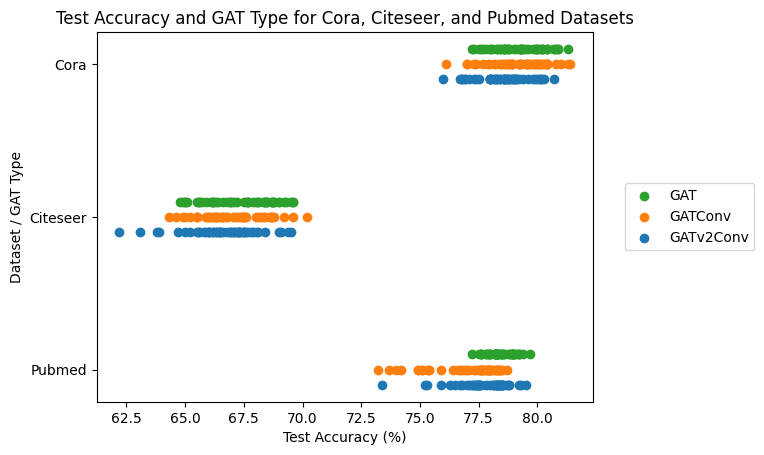
\includegraphics[width=\textwidth, height=9cm]{images/Benchmarking_Result_Graph}
    \caption{Benchmarking Results for Various datasets for every GAT types used.}
    \label{fig:benchmarks}
\end{figure*}
As we can see, from comparing Table~\ref{tab:results-table} with the results from the paper,
our Cora and Citeseer results are slightly worse than the Cora and Citeseer results from the paper.
In the case of Pubmed, our results are quite a bit worse, with our best runs being
a little worse than the average from the paper, and our worse results being
a lot worse as seen in Figure~\ref{fig:benchmarks}.

\subsection{Results: PPI}\label{subsec:results:-ppi}
Training the model on the PPI data has proven to be significantly slower than
on the other datasets. We only ran the PPI data through the implementation
using the Pytorch Geometric GAT class, and ended up discarding our results
because the GAT class isn't flexible enough to accommodate the paper's
architecture, and we figured we would get back to this, which we unfortunately
didn't. The PPI data took roughly 16 hours to run on one of our machines and
made the machine essentially unusable during those 16 hours, and ran out of
memory when we tried to run it on another machine.

\begin{table}
    \centering
    \begin{tabular}{@{}llll@{}}
        \toprule
        \textbf{Dataset} & \textbf{GAT Type} & \textbf{Mean} & \textbf{Std. Dev.}\\
        \midrule
        Cora             &  {GAT}            &  {78.99}\%      & {1.13}\%             \\
        Cora             &  {GATConv}        &  {78.86}\%      & {1.15}\%             \\
        Cora             &  {GATv2Conv}      &  {78.53}\%      & {1.04}\%             \\
        Citeseer         &  {GAT}            &  {67.01}\%      & {1.43}\%             \\
        Citeseer         &  {GATConv}        &  {66.83}\%      & {1.41}\%             \\
        Citeseer         &  {GATv2Conv}      &  {66.65}\%      & {1.47}\%             \\
        Pubmed           &  {GAT}            &  {77.73}\%      & {1.11}\%             \\
        Pubmed           &  {GATConv}        &  {77.38}\%      & {1.32}\%             \\
        Pubmed           &  {GATv2Conv}      &  {77.73}\%      & {1.22}\%             \\
        \bottomrule

    \end{tabular}
    \caption{Results using various GAT implementations. Each dataset was executed with each GAT type 50 times
    and the Mean and Standard deviation results was taken}
    \label{tab:results-table}
\end{table}

\subsection{Results: Pytorch implementation}\label{subsec:results:-pytorch-implementation}
We also tried writing our own implementation of the GAT model using Pytorch
primitives. The idea was to gain a deeper understanding of the model and to be
able to experiment more flexibly with the model, since we can control
everything in the model with an implementation written from scratch, whereas
there are aspects of the model that we can't control when using Pytorch
Geometric's classes.

Unfortunately, both our attempts are rewriting GAT using Pytorch failed. We
first tried to translate the implementation written by the paper's authors~\cite{petarvgatgithub} from Tensorflow to Pytorch, but its
accuracy stopped increasing on the training data at roughly 50\% accuracy. This
is in stark contrast to the previously-discussed implementations which achieved
well over 80\% accuracy on the training data.

We then used~\href{https://github.com/gordicaleksa/pytorch-GAT/blob/main/models/definitions/GAT
.py#L349}{\textit{another Pytorch implementation we found online}} as a reference for another Pytorch
GAT implementation.
Similarly to the previous attempt, training accuracy stopped increasing around 45\% accuracy.

\subsection{Ablation Results}\label{subsec:ablation-results}
Lastly, we ran the Cora, Citeseer and Pubmed datasets through three
architectural variants of the model. In two cases, we wrote single-layer
GAT implementations, and the other was a three-layer GAT implementation.
The results for all the ablations are shown in the Table~\ref{tab:ablation-results}.
\begin{table}
    \centering
    \begin{tabular}{@{}llll@{}}
        \toprule
        \textbf{Model Type}     & \textbf{Dataset}   & \textbf{Accuracy}\\
        \midrule
        Single Layer GAT (v1)   &  {Cora}            &  {73.20}\%    \\
        Single Layer GAT (v2)   &  {Citeseer}        &  {62.70}\%    \\
        Three Layer GAT         &  {Pubmed}          &  {70.40}\%    \\
        \bottomrule

    \end{tabular}
    \caption{Results for various ablations in the GAT implementation.}
    \label{tab:ablation-results}
\end{table}
